\documentclass[12pt, letterpaper]{article}
\usepackage[margin=1in]{geometry} % standard is 1.5inch
\usepackage{graphicx}
\usepackage{caption}
\usepackage{amsmath}
\usepackage{amsthm}
\usepackage{bbm}
\usepackage{tikz}
\usepackage[title]{appendix}
\usepackage{hyperref}
\usetikzlibrary{patterns}
%\usepackage{stix}
\usepackage{amssymb}
\usepackage{enumitem}
\title{Thesis Rough Work}
\author{Justin Furlotte (Student \#: 64238736)}
\date{June 17, 2021}
\begin{document}
\begin{titlepage}
\maketitle
\end{titlepage}

\newtheorem{theorem}{Theorem}
\newtheorem{corollary}{Corollary}
\newtheorem{lemma}{Lemma}
\newtheorem{proposition}{Proposition}
\newtheorem{assumption}{Assumption}
 
\newcommand{\C}{\mathbb{C}}
\newcommand{\Tr}{\text{Tr}}
\newcommand{\eps}{\varepsilon}
\newcommand{\R}{\mathbb{R}}
\newcommand{\N}{\mathbb{N}}
\newcommand{\Z}{\mathbb{Z}}
\newcommand{\norm}[1]{\lVert #1 \rVert}
\newcommand{\One}{\mathbbm{1}}
\newcommand{\Var}{\text{Var}}
\newcommand{\F}{\mathcal{F}}
\newcommand{\G}{\mathcal{G}}
\newcommand{\U}{\mathcal{U}}


\graphicspath{ {c:/user/justin/grad school/Thesis} }

\section{Setting}

Let $L\in\N$, and let $\Lambda_L = \Z_L \times [0,L]$ be the discrete cylinder, equipped with a metric $d$. To each site $x \in \Lambda_L$, we associate a Hilbert space $\mathcal{H}_x$ whose dimension is bounded uniformly in $L$, i.e. there exists some $N>0$ such that for all $L \in \N$, we have $\text{dim}(\mathcal{H}_x) \leq N$ for all $x \in \Lambda_L$. For a subset $X \subseteq \Lambda_L$, we define the Hilbert space $\mathcal{H}_X = \otimes_{x \in X} \mathcal{H}_x$, and we set $\mathcal{H}_L := \mathcal{H}_{\Lambda_L} = \otimes_{x \in \Lambda_L}\mathcal{H}_x$. For simplicity, throughout we take $L = 2^n$ for some large $n$.

The algebra $\U_L \subset \mathcal{B}(\mathcal{H}_L)$ of observables on $\Lambda_L$ is the set of bounded operators on $\mathcal{H}_L$ which are self-adjoint. For an operator $A_X \in \U_X$, we identify its extension to $\U_L$ by taking its tensor product with copies of the identity, $A_X \otimes_{x \in X^\mathsf{c}} \mathbb{I}_x$. Conversely, we say that an operator $A_X \in \Lambda_L$ has support $X$ if $A_X = A_X|_{X} \otimes_{x \in X^\mathsf{c}} \mathbb{I}_x$, and write $A_X \in \U_X$.

A \textit{local interaction} is a map $\Phi : \mathcal{P}(\Lambda_L) \to \U_L$ such that $\Phi(X) = 0$ whenever $\text{diam}(X) > R$, $\Phi(X)$ is supported in $X$, and $\norm{\Phi(X)} \leq C$ for all $X \subset \Lambda_L$, for all $L$.

We consider a region as depicted in Figure~\ref{fig:setup}. In the left white region $[0,L/2] \times [0,L]$, $H_0$ is a trivial Hamiltonian which we take to be the void (for example $H_0=0$), and in the right blue region $[L/2,L]\times [0,L]$, $H_1$ is a nontrivial \textit{local Hamiltonian}, in the sense that $H_1 = \sum_{X \subseteq \Lambda} \Phi(X)$, where $\Phi$ is a local interaction. We define the Hamiltonian of the full system to be 

\[H(\mu) = H_1 + \mu Q_h,\]

where $Q_h = \sum_{x \in \Gamma_h} a_x^*a_x$ is the number operator for the region $\Gamma_h = [L/4,3L/4] \times [0,L]$. 

\begin{figure}[h!]
\centering
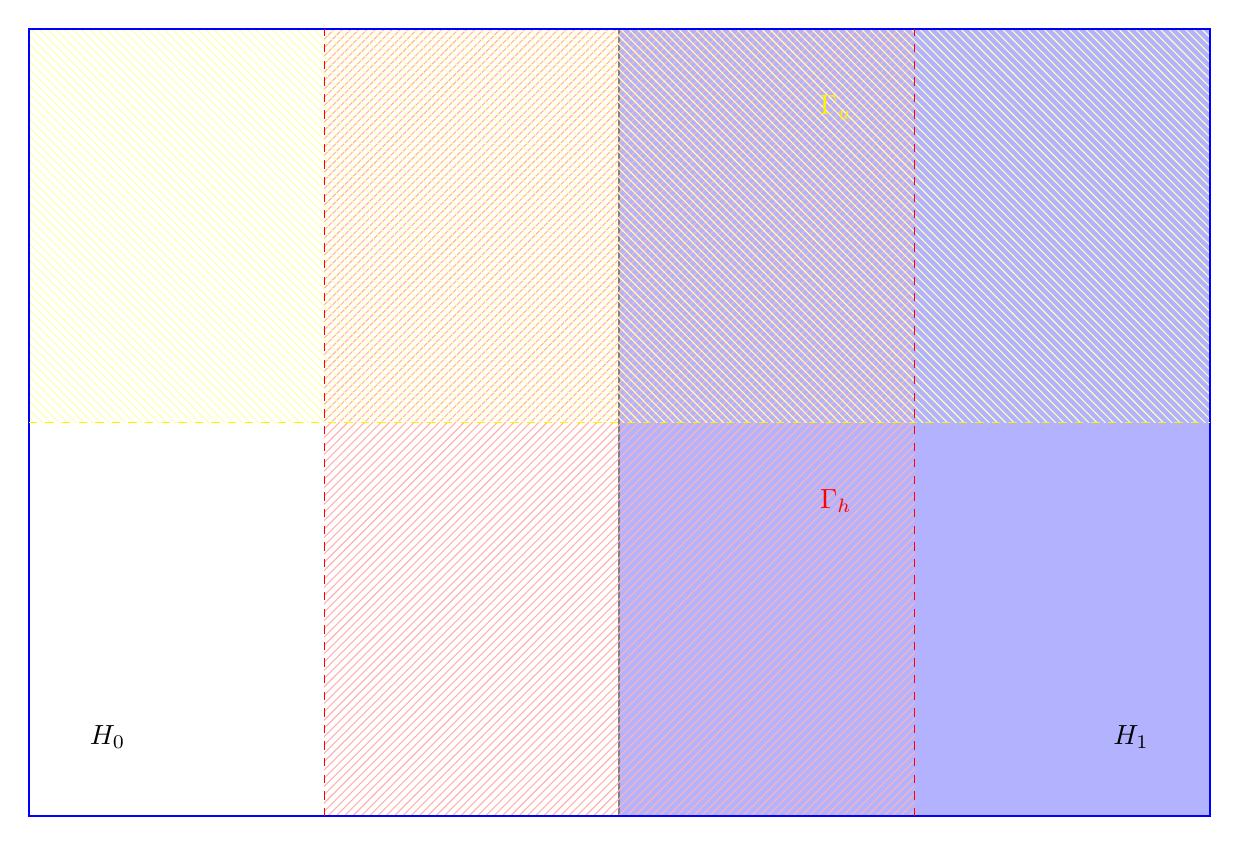
\begin{tikzpicture}
\fill[color=blue!30] (7.5,0) rectangle (15,10);
\draw[gray, thick] (7.5,0) -- (7.5,10);
\fill[pattern=north east lines, pattern color=red!30] (3.75,0) rectangle (11.25,10);
\fill[pattern=north west lines, pattern color=yellow!30] (0,5) rectangle (15,10);
\draw[blue, thick] (0,0) rectangle (15,10);
\draw[dashed, color=yellow] (0,5) -- (15,5);
\draw[dashed, color=red] (3.75,0) -- (3.75,10);
\draw[dashed, color=red] (11.25,0) -- (11.25,10);
\node[] at (1,1) {$H_0$};
\node[] at (14,1) {$H_1$};
\node[color=red] at (10.25,4) {$\Gamma_h$};
\node[color=yellow] at (10.25,9) {$\Gamma_u$};
\end{tikzpicture}
\caption{The setup for $\Lambda_L$. The left and right edges are identified to form a cylinder.}
\label{fig:setup}
\end{figure}

We also consider the plane $\Z^2$. In this setting, there are no edge states, and so the associated ``bulk" Hamiltonian $H_B(\mu)$ is assumed to have a \textit{gapped} spectrum, in the sense that

\begin{assumption}
\[\sigma(H_B) = \mathcal{S}_{-} \cup \mathcal{S}_{+},\]
where $\inf\mathcal{S}_{+} - \sup \mathcal{S}_{-} \geq \gamma$ uniformly in $L$ and $\mu$ for some $\gamma > 0$. 
\label{ass:gap}
\end{assumption}

In the case of the cylinder, this effect does not necessarily occur due to the presence of the edge. 
We also assume that the Hamiltonian is \emph{charge-conserving}.

\begin{assumption}
$[H(\mu), Q] = 0$, where $Q$ is the total charge in $\Lambda_L$.
\label{ass:charge}
\end{assumption}

Let $P_B$ be the ground state projection of $H_B$ (the system without an edge), and let $P$ be the ground state projection of $H$ (the system with an edge). We assume that states far from the edge are essentially bulk states, up to tails that vanish quickly in $L$.

\begin{assumption}
Define the bulk region $\Gamma_B = [L/2+k, L] \times [0,L]$ for some $k > 2R$. For any operator $A \in \U_{\Gamma_B}$,
\[\emph{Tr}(PA) = \emph{Tr}(P_BA) + \mathcal{O}(L^{-\infty}).\]
\label{ass:bulk}
\end{assumption}

(need to add justification)

For ease of notation, we omit the subscript $L$ wherever there is no risk of confusion.

\section{Equality of Bulk and Edge Currents}

\subsection{Cylinder Geometry}

Let $P(\mu)$ be the (possibly degenerate) ground state projection of $H(\mu)$. Let $Q_u = \sum_{x \in \Gamma_u} a_x^* a_x$ be the charge in the upper half of the cylinder $\Gamma_u = [0,L] \times [L/2,L]$, and define current operator 

\[J_u = i[H(\mu),Q_u].\]

For simplicity, we drop the subscript $u$ and simply write $J=J_u$. Charge conservation~\ref{ass:charge} implies that this current operator is supported on the strip $[L/2, L] \times [L/2-R, L/2+R]$, i.e. along a strip of width $2R$ centred at the line $y=L/2$. Indeed, if we inspect a local interaction $\Phi(X)$ of range $R$ with support $S \subset (\Gamma_u)_R$, where $(\Gamma)_\alpha$ is the $\alpha$-shrinking of $\Gamma$, then clearly $[\Phi(X), Q_u] = [\Phi(X), Q] = 0$, by assumption~\ref{ass:charge}. Similarly, if $\Phi(X)$ has support $S \subset ((\Gamma_u)^\mathsf{c})_R$, then $[\Phi(X), Q_u] = [\Phi(X), Q] = 0$. It follows that for an interaction $\Phi(X)$ with range $R$ and arbitrary support, $[\Phi(X), Q_u]$ must be supported on a set which is contained in (or equal to) the strip $[L/2, L] \times [L/2-R, L/2+R]$, and so $[H,Q_u]$ must be as well, since $H$ is a sum of such local interactions.

% In the case of a unique ground state $\Omega$, the total change in charge in $\Gamma_h$ after threading one quantum of flux is given by the fundamental theorem of calculus,

%\[ \int_{t:\Phi = 0}^{t:\Phi=2\pi} i[H, Q_u] dt' = \langle \Omega, (U^* Q_h U - Q_h) \Omega \rangle\]

\begin{lemma}
The ground state expectation of the current $J$ is zero.
\label{lemma:J=0}
\end{lemma}
\begin{proof}
By cyclicity of the trace and commutativity of $P(\mu)$ with $H(\mu)$, 
\[\begin{aligned}
\Tr(P(\mu) J) &= \Tr(P(\mu)i[H(\mu),Q_u]) \\
&= \Tr(iP(\mu)H(\mu)Q_u) - \Tr(iP(\mu)Q_u H(\mu))\\
&= \Tr(iH(\mu)P(\mu)Q_u) - \Tr(iH(\mu)P(\mu)Q_u)\\
&=0.
\end{aligned}\]
\end{proof}

Define the operators

\[K(\mu) = \mathcal{I}_{\mu}(\dot{H}(\mu)),\]

where 

\[\mathcal{I}_{\mu} (A) = \int_\R W(t) e^{itH(\mu)} A e^{-itH(\mu)}dt.\]

More explicitly, in this setting we see that $K(\mu) = \mathcal{I}_\mu(Q_h)$. As a shorthand, we use the notation $\dot{A}(\mu_0)= \frac{d}{d\mu}A|_{\mu_0}$. 

We present two important properties of the map $\mathcal{I}_\mu$ in the following lemmas, and leave their proofs to the appendix (need to add). We will also need a definition: an \emph{off-diagonal} operator is an operator $A$ such that $A = \overline{A} := PAP^\perp + P^\perp AP$, where $P^\perp = \mathbb{I} - P$ is the projection onto the excited states above the gap.

\begin{lemma}
For any off-diagonal operator $A$, $\mathcal{I}_\mu(\cdot)$ and $[H(\mu), \cdot]$ act as inverses of each other, up to a factor of $i$:

\[\mathcal{I}_\mu\left([H(\mu), A]\right) = [H(\mu), \mathcal{I}_\mu(A)] = iA\]
\label{lemma:inverseofH}
\end{lemma}

It is easy to verify that any operator $A$ behaves as an off-diagonal operator when taking a commutator with $P$, in the sense that

\[[\overline{A}, P] = [PA(1-P) + (1-P)AP, P] = [A,P].\]

It follows that for any (not necessarily off-diagonal) operator $A$, 

\[[\mathcal{I}([H, A]),P] = i[A,P]\]

\begin{lemma}
$\mathcal{I}_\mu$ is local in the sense that for any $A \in \mathcal{U}_X$, 

\[\norm{\mathcal{I}(A)_{(X^r)^\mathsf{c}}} \leq \norm{A} |X| \mathcal{O}(r^{-\infty}).\]
\label{lemma:local}
\end{lemma}

\begin{proposition}
The operator $K(\mu)$ is the \emph{generator of parallel transport}, satisfying
\[\dot{P}(\mu) = i[K(\mu),P(\mu)].\]
\label{prop:generatorparalleltransport}
\end{proposition}
\begin{proof}
By the product rule and the fact that $H(\mu)$ and $P(\mu)$ commute, 

\[ [\dot{H}(\mu), P] = -[H, \dot{P}(\mu)]. \]

Now we show that $\dot{P}(\mu)$ is off-diagonal. Taking the derivative on both sides of $P^2=P$, we see that $\dot{P}P + P\dot{P} = \dot{P}$. Acting on the left and right with $P$ on both sides of this equation gives 

\[P\dot{P}P + P\dot{P}P = P\dot{P}P,\]

which implies that $P\dot{P}P = 0$. Now, 

\[\begin{aligned}
\overline{\partial_\mu P} &= P(\partial_\mu P)(1-P) + (1-P)(\partial_\mu P)P\\
&= P(\partial_\mu P) - P(\partial_\mu P)P + (\partial_\mu P)P - P(\partial_\mu P)P\\
&= P(\partial_\mu P) + (\partial_\mu P)P\\
&= \partial_\mu (P^2)\\
&= \partial_\mu P,
\end{aligned}\]

as claimed. It therefore follows from Lemma~\ref{lemma:inverseofH} that

\[\begin{aligned}
\dot{P}(\mu) &= -i \mathcal{I}_\mu([H(\mu), \dot{P}(\mu)])\\
&= i\mathcal{I}_\mu([\dot{H}(\mu), P(\mu)])\\
&= i[\mathcal{I}_\mu(\dot{H}(\mu)), P(\mu)]\\
&= i[K(\mu), P(\mu)].
\end{aligned}\]
\end{proof}

Increasing the ``electric potential" by a small amount $d\mu Q_h$ and expanding to linear order, the change in ground state current is given by

\[\Tr(P(\mu+d\mu)J) - \Tr(P(\mu)J) = \kappa d\mu + \mathcal{O}(d\mu^2).\]

Dividing by $d\mu$ and taking a limit, we see that the linear response coefficient is given by

\[\kappa = \Tr\left(\dot{P}(\mu) J\right).\]

The \emph{Hall conductivity} of the system on a subset $V \subseteq \Lambda$ is defined to be $\kappa_V := \Tr\left(\dot{P}(\mu) J_V\right)$, where $J_V$ is the restriction of the operator $J$ to $V$. 

\begin{proposition}
The Hall conductivity is independent of the driving strength $\mu$.
\end{proposition}
\begin{proof}
We see by cyclicity of the trace and the formula $\dot{H}(\mu)=Q_h$ that for any $\mu_1$ and $\mu_2$,

\[\begin{aligned}
\kappa(\mu_1) - \kappa(\mu_2) &= \Tr\left( \dot{P}(\mu_1) i[H(\mu_1), Q_u] - \dot{P}(\mu_2)i[H(\mu_1),Q_u]\right)\\
&= i\Tr\left(\left([\dot{P}(\mu_1), H(\mu_1)] - [\dot{P}(\mu_2), H(\mu_2)]\right)Q_u\right)\\
&= i\Tr\left( \left([\dot{H}(\mu_1), P(\mu_1)] - [\dot{H}(\mu_2), P(\mu_2)]\right)Q_u \right)\\
&= i\Tr\left( [Q_h, P(\mu_1) - P(\mu_2)]Q_u \right)\\
&= i\Tr \left( Q_h(P(\mu_1) - P(\mu_2))Q_u - (P(\mu_1)-P(\mu_2))Q_uQ_h \right)\\
&= 0,
\end{aligned}\]

since $Q_h$ and $Q_u$ commute, indicating that the Hall conductivity is independent of $\mu$ as one would expect physically.
\end{proof}

The following is the main result:

\begin{theorem}
The ground state current in the strip $[L/2+k, 3L/4-k] \times [0,L]$ between the edge and the bulk current vanishes, in the sense that $\kappa_V = \mathcal{O}(r^{-\infty}) + \mathcal{O}(L^{-\infty})$ for any $V \subseteq [L/2+R, 3L/4-R] \times [0,L]$ ``in between" the bulk and edge strips, where 

\[r = \emph{dist}(V, [L/2-R, 3L/4+R] \times [0, L] \cup [3L/4-R, 3L/4+R] \times [0, L])\]

is the distance from $V$ to one of the edge or bulk strips.

\end{theorem}

\begin{proof}
By Proposition~\ref{prop:generatorparalleltransport}, the Hall conductivity can also be written by the formula $\kappa_V^B = \Tr\left(i[K(\mu),P_B(\mu)]J_V^B\right) = \Tr\left(i[\mathcal{I}_\mu(Q_h), P_B(\mu)]J_V^B\right)$, where $J_V^B = \left(i[H_B, Q_u]\right)_V$ is the current arising from the bulk Hamiltonian. From commutativity of $P_B$ and $H_B$ along with cyclicity of the trace, we compute

\[\begin{aligned}
\kappa_V^B &= \Tr\left(i[\mathcal{I}_\mu(Q_h), P_B(\mu)]J_V^B\right)\\
&= \Tr\left(i\int_\R W(t) e^{itH_B(\mu)} [Q_h,P_B(\mu)] e^{-itH_B(\mu)}dt J_V^B \right)\\
&= \int_\R W(t) \Tr\left(i[Q_h,P_B(\mu)] e^{-itH_B(\mu)}J_V^Be^{itH_B(\mu)}\right)dt\\
&= -\int_\R W(t) \Tr\left(i[Q_h,P_B(\mu)] e^{itH_B(\mu)}J_V^Be^{-itH_B(\mu)}\right)dt\\
&=- \Tr\left(i[Q_h,P_B(\mu)]\mathcal{I}_\mu(J_V^B)\right),
\end{aligned}\]

since $W(t)$ is odd. Again by cyclicity of trace combined with the fact that $\mathcal{I}_\mu(\cdot)$ is an inverse of $[H_B(\mu), \cdot]$ for commutators with $P_B(\mu)$ (by the remark after lemma~\ref{lemma:inverseofH}), we obtain

\[\begin{aligned}
\kappa_V^B &=-\Tr([\mathcal{I}_\mu([H_B(\mu),Q_h]), P_B(\mu)]\mathcal{I}_\mu(J_V^B))\\
&=-\Tr(\mathcal{I}_\mu([H_B(\mu),Q_h]) P_B(\mu)\mathcal{I}_\mu(J_V^B) - P_B(\mu) \mathcal{I}_\mu([H_B(\mu),Q_h])\mathcal{I}_\mu(J_V^B)) )\\
&=-\Tr(P_B(\mu)\mathcal{I}_\mu(J_V^B) \mathcal{I}_\mu([H_B(\mu),Q_h]) - P_B(\mu) \mathcal{I}_\mu([H_B(\mu),Q_h])\mathcal{I}_\mu(J_V^B)) )\\
&= \Tr\left( P_B(\mu)[\mathcal{I_\mu}([H_B(\mu),Q_h]), \mathcal{I}_\mu(J_V^B)]\right).
\end{aligned}\]

Now, $[H_B(\mu), Q_h]$ is a local operator, supported on the ``bulk line" $[3L/4-R, 3L/4+R] \times [0, L]$, while $J_V^B$ is a local operator supported on $V \subseteq [L/2+k, 3L/4-k] \times [0,L]$. Since $\mathcal{I}_\mu$ preserves locality up to tails, in the sense that $\norm{\mathcal{I}_\mu(A)_{(S^r)^\mathsf{c}}} \leq \norm{A} |S| \mathcal{O}(r^{-\infty})$ (Lemma~\ref{lemma:local}), it follows that the commutator $[\mathcal{I_\mu}([H_B(\mu),Q_h]), \mathcal{I}_\mu(J_V^B)] = C\mathcal{O}(r^{-\infty})$ whenever $V \cap ([3L/4-R, 3L/4+R] \times [L/2, L]) = \varnothing$.

The previous fact applies to the bulk setting with $H_B$ and $P_B$. To extend this to the setting with an edge, it is enough to use Assumption~\ref{ass:bulk} to conclude the same result, except with equality up to $\mathcal{O}(L^{-\infty})$, i.e.

\[\kappa_V = \Tr\left(\dot{P}J_V\right) = \Tr\left(\dot{P}(J_V^B + \mathcal{O}(L^{-\infty}))\right) = \kappa_V^B + \mathcal{O}(L^{-\infty}) = \mathcal{O}(r^{-\infty}) + \mathcal{O}(L^{-\infty}).\]

\end{proof}


The intuitive picture from the previous result is that, in the bulk region, the Hall conductivity is essentially only nonzero along  the bulk line $[3L/4-R, 3L/4+R] \times [L/2, L]$. Since the ground state expectation of the current is zero (by lemma~\ref{lemma:J=0}), it must be that there is an equal current flowing along the edge, but in the opposite direction, see figure (need to add).

\subsection{Torus Geometry}

Our goal is to show the same result on the discrete torus $\mathbb{T}_L := \Z_L \times \Z_L$. We define the same regions $\Gamma_u$ and $\Gamma_h$, and the same current operator $J_u = i[H(\mu), Q_u]$. This time, however, Lemma~\ref{lemma:J=0} does not apply. Intuitively, it does not apply because electrons can now flow through both the bottom and the top of the region $\Gamma_u$, rather than just the bottom. Mathematically, the lemma fails because our definition of the current is slightly changed.

We use charge conservation and the fact that $H$ is finite range to split the current $J_u$ into two components, $J_u = i[H_-, Q_u] + i[H_+, Q_u] = J_- - J_+$, supported on strips of width $2R$ at $y=L/2$ and $y=L$, respectively. We then define the current operator to be $J=J_-$, which is the current on the lower strip. This is the mathematical reason that the proof in Lemma~\ref{lemma:J=0} fails on the torus; we have replaced $H$ by $H_-$, which may no longer commute with $P$. We instead proceed by a different approach. We will need a few auxiliary results first.

\begin{lemma}
$K_\pm$ is supported on $\partial_\pm$ up to tails.
\label{SupportOfK}
\end{lemma}
\begin{proof}

\end{proof}

\begin{proposition}
The operator $Q_h-K$ leaves the ground state space invariant, i.e. $[Q_h-K, P] = 0$.
\end{proposition}
\begin{proof}

\end{proof}


\begin{lemma}
Show that $\emph{Tr}(A,[Q_h,P])=0$ for all $A \in \mathcal{U}_{\text{edge}}$. This shows that $Q_h$ commutes with $P$ ``along the edge".
\label{lemma:[Q,P]=0}
\end{lemma}
\begin{proof}

Let $A \in \mathcal{U}_{\text{edge}}$. Since $H$ is charge conserving, we may choose a simultaneous eigenbasis of $H$ and the total charge $Q$, in which case $P$ and $Q$ commute. It follows that

\[\begin{aligned}
\Tr(A[Q_h, P]) = \Tr([A, Q_h] P) = \Tr([A, Q]P) = \Tr(A[Q,P]) = 0.
\end{aligned}\]



%\[\begin{aligned}
%\Tr(A [Q_h, P]) &= \Tr([A, Q_h]P)\\
%&= \Tr([P,A]Q_h)\\
%&= \sum_{x \in \Gamma_h} \Tr([P, A] c_x^*c_x)\\
%&= \sum_{x \in \Gamma_h} \Tr\left(\bigotimes_{y \in \text{supp}([P, A])} \left[P, A\right]_y c_x^*c_x\right)\\
%&= \sum_{x \in \Gamma_h} \Tr\left(\bigotimes_{y \in \text{supp}([P, A])} \left[P_y, A_y\right] c_x^*c_x\right)\\
%&= \sum_{x \in \Gamma_h} \prod_{y \in \text{supp}([P, A])} \Tr([P_y, A_y] c_x^*c_x)
%\end{aligned}\]

%The support of $[P, A]$ is the edge, so

%\[\begin{aligned}
%\Tr(A [Q_h, P]) &= \sum_{x \in \Gamma_h} \prod_{y \in \text{edge}} \Tr([P_y, A_y] c_x^*c_x)\\
%&= \sum_{x \in \Gamma_h} \prod_{y \in \text{edge}} \Tr((\mathbb{I}\otimes\ldots\otimes\mathbb{I}\otimes [P_y, A_y] \otimes\mathbb{I}\ldots\otimes\mathbb{I}) (\mathbb{I}\otimes \ldots \otimes\mathbb{I} \otimes c^*_xc_x \otimes \mathbb{I} \ldots\otimes\mathbb{I}))\\
%&= \sum_{x \in \Gamma_h} \prod_{y \in \text{edge}} \Tr(\mathbb{I}\otimes\ldots\otimes\mathbb{I}\otimes c_x^*c_x \otimes \mathbb{I} \otimes \ldots \otimes\mathbb{I} \otimes [P_y, A_y] \otimes\mathbb{I}\ldots)\\
%&= \sum_{x \in \Gamma_h} \prod_{y \in \text{edge}, \; y\neq x} \Tr(c_x^*c_x)\Tr([P_y, A_y]) + \sum_{x \in \Gamma_h \cap \text{edge}} \Tr(c_x^*c_x [P_x, A_x]).\\
%\end{aligned}\]

%Since the trace of any commutator is zero, the terms in the first sum vanish. Since $\Gamma_h \cap \text{edge} =\text{edge}$, we are left with

%\[\Tr(A[Q_h, P]) = \sum_{x \in \text{edge}} \Tr(c_x^*c_x[P_x, A_x]) = \sum_{x \in \text{edge}} \Tr(P_x[A_x, c_x^*c_x]).\]

%For any particular $x\in \text{edge}$, write $P_x = \sum_n |\psi_n \rangle \langle \psi_n |$, where the sum is over ground states, and 

%\[\langle \psi | [P_y, A_y]|\psi\rangle = \sum_n \langle \psi | \psi_n \rangle \langle\psi_n | A |\psi\rangle - \sum_n \langle \psi | A |\psi_n\rangle\langle\psi_n | \psi\rangle \]

%Want to show:

%\[\Tr([P_y, A_y]) = \ldots = 0\]

\end{proof}

Finally, we will prove that in the bulk system with Hamiltonian $H_B(\mu)$, the ground state expectation of the current vanishes faster than any power as $L \to \infty$.

\begin{lemma}
The ground state expectation of the current $J_B := i[(H_B)_-, Q_h]$ (of the system without an edge) is $\emph{Tr}(P_BJ_B)=\mathcal{O}(L^{-\infty})$.
\label{J=0Bulk}
\end{lemma}
\begin{proof}
First, $K = \mathcal{I}(i[H_B, Q])$ splits into $K = K_- - K_+$, with the support of $K_\pm$ contained in $\partial_\pm$ up to tails:

\[[K_\pm, A_X] = \mathcal{O}(p^{-\infty}),\]

for every $A_X \in \mathcal{U}_X$ such that $\norm{A_X}=1$, and where $p = \text{dist}(X, \partial_\pm)$ (need to add). Using the fact that $K_\pm$ is supported in $\partial_\pm$ up to tails (Lemma~\ref{SupportOfK}), we see that 

\[i[H_B, K_-] = i[(H_B)_-, K_-] + \mathcal{O}(L^{-\infty}),\]

and similarly $i[(H_B)_-, K_+] = \mathcal{O}(L^{-\infty})$. Putting these facts together, it follows that the current can be rewritten as 

\[\begin{aligned} 
J _B&= i[H_B, Q_h + K_- - K_- + K_+] + \mathcal{O}(L^{-\infty})\\
&= i[H_B, K_-] + i[(H_B)_-, Q_h - K_- + K_+)] + \mathcal{O}(L^{-\infty}).
\end{aligned}\]

From here, we use the fact that $H_B$ and $Q_h-K_-+K_+$ both commute with $P_B$ to write

\[P_BJ_BP_B = i[H_B, P_BK_-P_B] + i[P_B(H_B)_-P_B, Q_h - K_- + K_+)] + P_B\mathcal{O}(L^{-\infty})P_B.\]

Since the trace of any commutator is zero, 

\[\Tr(P_BJ_B) = \Tr(P_BJ_BP_B) = \mathcal{O}(L^{-\infty}).\]

\end{proof}

Using this, we can show a simple proof of the analogue of Lemma~\ref{lemma:J=0} on the torus, in the case of non-interacting systems.

\begin{proposition}
Let $H = \sum_{x \in \mathbb{T}} h_x$ be a non-interacting Hamiltonian, i.e. a sum of single site Hamiltonians $h_x$. The ground state expectation of the current $J=i[H_-, Q_h]$ (of the system with an edge) is $\emph{Tr}(PJ)=\mathcal{O}(L^{-\infty})$.
\label{prop:J=0Torus}
\end{proposition}

\begin{proof}

Since $H$ is a sum of single site Hamiltonians, we can split $H_-$ into the restrictions $H_- = (H_-)_\text{edge} + (H_-)_\text{bulk}$, with no fear of any terms which are in both the edge region and the bulk region. By Assumption~\ref{ass:bulk},

\[\begin{aligned}
\Tr(PJ) &= \Tr(Pi[H_-, Q_h])\\
&= i\Tr([H_-, Q_h]P)\\
&= i\Tr((H_-)_\text{edge} [Q_h, P]) + i \Tr((H_-)_\text{bulk} [Q_h, P])\\
&= i\Tr((H_-)_\text{edge} [Q_h, P]) + i \Tr((H_-)_\text{bulk} [Q_h, (P)_\text{bulk}])\\
&= i\Tr((H_-)_\text{edge} [Q_h, P]) + i \Tr((H_B)_-[Q_h, P_B]) + \mathcal{O}(L^{-\infty})\\
&= i\Tr((H_-)_\text{edge} [Q_h, P]) + \Tr(i[(H_B)_-, Q_h]P_B) + \mathcal{O}(L^{-\infty}).
\end{aligned}\]

By Lemma~\ref{lemma:[Q,P]=0}, the first term is zero. By Lemma~\ref{J=0Bulk}, the second term is $\mathcal{O}(L^{-\infty})$. 
\end{proof}

\newpage
\appendix

\section{Properties of $\mathcal{I}_\mu$}

\begin{proof}
(Of Lemma~\ref{lemma:inverseofH}). Let $\widehat{W}(\xi) = \frac{1}{\sqrt{2\pi}}\int_\R W(t) e^{-2\pi i t \xi} dt$ be the Fourier transform of $W$. One can show that for $|\xi|\geq \gamma$, $\widehat{W}(\xi) = \frac{1}{\sqrt{2\pi}i \xi}$ (need to add). Let $A$ be an observable. First, we show that $\mathcal{I}([H,PAP^\perp]) = iPAP^\perp$. 

Decomposing 

\[\begin{aligned}
e^{itH}P &= \sum_{j=0}^\infty \frac{(itH)^j}{j!} P \\
&= \sum_{j =0}^\infty \frac{(it)^j}{j!} \left(\sum_n E_n^j P_n\right)P \\
&= \sum_{j=0}^\infty \frac{(it)^j}{j!} \sum_{n : E_n=0} E_n^j P_n \\
&= \sum_{n : E_n=0} e^{itE_n}P_n,
\end{aligned}\]

and similarly 

\[P^\perp e^{-itH}= \sum_{m:E_m \geq \gamma}P_m e^{-itE_m},\]

we see that

\[\begin{aligned}
\mathcal{I}([H,PAP^\perp]) &= \mathcal{I}(P[H,A]P^\perp) \\
&= \int_\R W(t)e^{itH}P[H,A]P^\perp e^{-itH}dt \\
&= \int_\R W(t) \sum_{n : E_n=0} e^{itE_n}P_n [H,A] \sum_{m:E_m \geq \gamma} P_m e^{-itE_m} dt\\
&= \sum_{n : E_n=0} \sum_{m:E_m \geq \gamma} \int_\R W(t) e^{itE_n} P_n A (E_n-E_m) P_m e^{-itE_m}dt\\
&= \sum_{n : E_n=0} \sum_{m:E_m \geq \gamma} P_n A P_m (E_n-E_m) \int_\R W(t) e^{-it(E_m - E_n)} dt\\
&= \sum_{n : E_n=0} \sum_{m:E_m \geq \gamma} P_n A P_m (E_n-E_m) \sqrt{2\pi} \widehat{W}(E_m-E_n) \\
&= i\sum_{n : E_n=0} \sum_{m:E_m \geq \gamma} P_n A P_m\\
&= iPAP^\perp.
\end{aligned}\]

(need to check the $2\pi$ factor)

By the same argument, $\mathcal{I}([H,P^\perp AP]) = iP^\perp AP$ as well, and so $\mathcal{I}([H,\overline{A}]) = i\overline{A}$.
\end{proof}

\begin{proof}

(Of Lemma~\ref{lemma:local}). We break the integral into two parts,

\[\norm{\mathcal{I}(A)} \leq \bigg\lVert\int_{-T}^T W(t) e^{itH}Ae^{-itH}dt \bigg\rVert + \bigg\lVert \int_{\R\setminus [-T,T]} W(t) e^{itH}Ae^{-itH}dt\bigg\rVert.\]

The first term can be estimated using the Lieb-Robinson bound found in Appendix~\ref{sec:L-R}.

\end{proof}

\section{Lieb-Robinson Bound}
\label{sec:L-R}

Let $N$ be a uniform upper bound for the dimensions of the Hilbert spaces at each site, i.e. $\text{dim}(\mathcal{H}_x) \leq N$ for all sites $x$.

The following is a version of the Lieb-Robinson. For any operators $A \in \mathcal{U}_X$ and $B \in \mathcal{U}_Y$ having disjoint supports $X\cap Y = \varnothing$, 

\[\norm{ [e^{itH}Ae^{-itH}, B] } \leq  C \norm{A}\norm{B} |X| |Y| N^{2|X|} e^{2t\norm{\Phi}_\lambda - \lambda d(X, Y)}.\]

\section{Gr\"{o}nwall's Inequality and Uniqueness}

\begin{theorem}
(Gr\"{o}nwall's Inequality). Let $\alpha : I \to (0,\infty)$ be positive and continuous on $I^o$ for some interval of the form $[a,b)$, $[a,b]$, or $[a,\infty)$. Suppose $u : \mathbb{R} \to \mathcal{U}$ is a Banach-valued, differentiable function. If $\norm{u'(t)} \leq \alpha(t)\norm{u(t)}$ for all $t\in I$, then 
\[\norm{u(t)} \leq \norm{u(a)} e^{\int_a^t \alpha(s)ds} \quad \forall t\in I\]
\end{theorem}
\label{thm:gronwallinequality}
\begin{proof}
Let $f(t) = e^{\int_a^t \alpha(s)ds}$, which is nonzero, has initial value $f(a)=1$, and has derivative $f'(t) = \alpha(t) f(t)$. Then by the quotient rule,
\[\left(\frac{\norm{u(t)}}{f(t)}\right)' = \frac{\norm{u'(t)}f(t) - \norm{u(t)}\alpha(t)f(t)}{f(t)^2} \leq 0,\]
where the inequality follows from the assumption $\norm{u'(t)} \leq \norm{\alpha(t)u(t)}$. Thus $\frac{\norm{u(t)}}{f(t)}$ is decreasing, so that 
\[\frac{\norm{u(t)}}{f(t)} \leq \frac{\norm{u(a)}}{f(a)} = \norm{u(a)},\]
which is the desired inequality.
\end{proof}

\begin{theorem}
(ODE Uniqueness). Let $F:\mathcal{U}\to\mathcal{U}$ be Lipschitz and consider the differential equaton $u'(t)=F(u(t))$ with initial condition $u(a) = u_a$ for some function $u:I\to\mathcal{U}$, where $I = [a,b]$, or $[a,b)$, or $[a,\infty)$. Solutions to this equation are unique.
\end{theorem}
\label{thm:gronwalluniqueness}
\begin{proof}
Suppose there are two solutions $u(t)$ and $v(t)$, and let $g(t) = \norm{u(t)-v(t)}^2$. By assumption, there exists a constant $L_F$ such that $\norm{F(u(t))-F(v(t))} \leq L_F \norm{u(t)-v(t)}$, so that
\[\begin{aligned}
g'(t) &= 2\norm{u(t)-v(t)}\norm{u'(t)-v'(t)}\\
&=2\norm{u(t)-v(t)}\norm{F(u(t))-F(v(t))}\\
&\leq 2L_F\norm{u(t)-v(t)}^2\\
&= 2L_F g(t).
\end{aligned}\]
Notice that $\alpha := 2L_F$ is a positive continuous function, so we may apply Gr\"{o}nwall's inequality to $g(t)$ to conclude
\[g(t) \leq g(a)e^{2L_f(t-a)} = 0,\]
since $g(a)=0$.
\end{proof}

\section{Note on Generators of Parallel Transport}
Consider the differential equation $\dot{\rho}(\mu) = i[K_B,\rho(\mu)]$ with initial condition $\rho(0)=P_B(0)$. Here $K_B = \int_\mathbb{R}W_\gamma(t)e^{-itH_B}\dot{H_B}e^{itH_B}dt$, and recall that in our setting, $\dot{H_B} = Q_h$. We know that the solution is $\rho(\mu) = P_B(\mu)$ (proposition \ref{prop:generatorparalleltransport}). Notice that the map $F:\mathcal{U}\to\mathcal{U}$ defined by $F(A) = i[K_B,A]$ is Lipschitz, since
\[\norm{F(A)-F(B)} = \norm{[K_B,A-B]} \leq 2\norm{K_B}\norm{A-B}.\]
The Lipschitz constant is $2\norm{K_B}$, which is finite since $K_B$ is a bounded operator:

\[\begin{aligned}
\norm{K_B} &\leq \int_\mathbb{R}|W_\gamma(t)| \norm{e^{-itH_B}Q_he^{itH_B}}dt\leq \int_\mathbb{R}|W_\gamma(t)|dt\norm{Q_h}.
\end{aligned}\]

Indeed, since $Q_h$ is the number operator on a finite volume, by charge conservation and the fact that the dimension of the Hilbert space is bounded uniformly by $d$, there can only be a finite number of charges in the region $\Gamma_h$.

Thus, by Gr\"{o}nwall's uniqueness theorem (appendix \ref{thm:gronwalluniqueness}), we see that the solution to the equation $\dot{\rho}(\mu) = F(\rho(\mu)) = i[K_B,\rho(\mu)]$ is unique. 

Now define 

\[K_E := \int_\mathbb{R} W_\gamma(t) e^{-itH_E}Q_he^{itH_E}dt,\]

which is using the gap $\gamma$ of $H_B$ to define $W_\gamma$, but also using the edge Hamiltonian in the time evolution operators. Consider $\sigma:[0,\infty)\to\mathcal{U}$ defined by

\[\dot{\sigma}(\mu) = i[K_E, \sigma(\mu)] \quad\quad\quad\quad \sigma(0) = P_B(0).\]

We now show that, similar to how $\rho$ is an approximation of $P_B$, $\sigma$ is also a good approximation of $P_E$ (up to $\mathcal{O}(L^{-\infty})$) ``in the bulk". Let $A\in \Gamma_B$ be an operator localized in the bulk of the edge system. Then 

\[\begin{aligned}
\Tr(\dot{\sigma} A) &= \Tr (i[K_E, \sigma]A)\\
&= \Tr(i[A,K_E]\sigma)\\
&= \int_\mathbb{R}W_\gamma(t) \Tr([e^{-itH_E}Q_he^{itH_E}, A] \sigma)dt\\
&= \int_\mathbb{R}W_\gamma(t) \Tr(e^{-itH_E}[Q_h, e^{itH_E}Ae^{-itH_E}]e^{itH_E} \sigma)dt\\
&= \int_\mathbb{R}W_\gamma(t) \Tr(e^{-itH_E}[Q_h, e^{itH_B}Ae^{-itH_B}]e^{itH_E} + \mathcal{O}(L^{-\infty})\sigma)dt\\
&= \int_\mathbb{R}W_\gamma(t) \Tr(e^{-itH_B}[Q_h, e^{itH_B}Ae^{-itH_B}]e^{itH_B} + \mathcal{O}(L^{-\infty})\sigma)dt\\
&= \int_\mathbb{R}W_\gamma(t) \Tr([e^{-itH_B}Q_he^{itH_B}, A] \sigma)dt + \mathcal{O}(L^{-\infty})\\
&= \Tr(i[A,K_B]\sigma] + \mathcal{O}(L^{-\infty})\\
&= \Tr(i[K_B,\sigma]A) + \mathcal{O}(L^{-\infty}),
\end{aligned}\]

since $\sigma$ is trace-class (?) and $W_\gamma \in L^1$. By linearity of the trace, we see that $\Tr((\dot{\sigma} - i[K_B,\sigma])A) = \mathcal{O}(L^{-\infty})$ for any operator $A \in \Gamma_B$ (does this mean $\dot{\sigma}-i[K_E,\sigma] = 0$?). But the solution of $\dot{\sigma} - i[K_B,\sigma] = 0$ (with initial condition $\sigma(0)=P_B(0)$) is unique; it is $\rho(\mu)$, or $P_B(\mu)$. Hence

\[\Tr(P_E A) = \Tr(P_B A) + \mathcal{O}(L^{-\infty}) = \Tr(\rho A) + \mathcal{O}(L^{-\infty}) = Tr(\sigma A) + \mathcal{O}(L^{-\infty}) \]

for any operator $A\in\Gamma_B$. In particular, this gives another local formula for the Hall conductivity in the bulk of an edge system, by taking $A = J_V$, where $J$ is the current operator and $V \subset \Gamma_B$ is a set localized in the bulk. The Hall conductivity is given by $\Tr(\dot{P_E}J_V)$, and this can be approximated by

\[\Tr(\dot{P_E} J_V) = \Tr(\dot{P_B} J_V) + \mathcal{O}(L^{-\infty}) = \Tr(\dot{\rho} J_V) + \mathcal{O}(L^{-\infty}) = \Tr(\dot{\sigma} J_V) + \mathcal{O}(L^{-\infty}).\]

Want to pick a norm s.t. Gronwall gives $\norm{\rho(\mu)-\sigma(\mu)}_G \leq \norm{P_B(0)-P_E(0)}_Ge^{2L_F\mu}$. Need $\norm{P_B(0)-P_E(0)}_G$ to be small enough to kill the exponential which depends on $L_F = 2\norm{K_B}_G \leq \norm{W_\gamma}_{L^1}\norm{Q_h}_G$. If we use the operator norm for $\norm{\cdot}_G$, we would get $\norm{Q_h}_G = d|\Gamma_h|$ in the exponent. Need $\norm{\cdot}_G$ to be an actual norm so that $\norm{\rho-\sigma}_G = 0 \implies \rho = \sigma$.

\end{document}